\section{Preventivo di Fase}
Si riporta nella seguente sezione il preventivo realizzato per la fase
di avanzamento "\textit{RTB}".\\
L'intento è quello di dividere equamente il lavoro tra i membri del gruppo,
così come descritto nella sezione \href{https://www.math.unipd.it/~tullio/IS-1/2021/Progetto/Capitolati.html}{\textit{"Organigramma fornitore"}}
presente nel sito di Ingegneria del Software, capitolo \textit{"Presentazione dei capitolati d'appalto"}.\\

\bigbreak
\noindent
I costi fissi stabiliti per ogni ruolo sono i seguenti:
\begin{table}[htb]
    \centering
    {\renewcommand{\arraystretch}{1.5}
    \begin{tabular}{cccc}
	    \rowcolor[RGB]{33, 73, 50}
	    \textcolor{white}{\textbf{Ruolo}} & \textcolor{white}{\textbf{Costo Orario}}\\
	    \rowcolor[RGB]{216, 235, 171}
	    Responsabile & 30\euro \\
	    \rowcolor[RGB]{233, 245, 206}
	    Amministratore & 20\euro\\
        \rowcolor[RGB]{216, 235, 171}
	    Analista & 25\euro\\
	    \rowcolor[RGB]{233, 245, 206}
	    Progettista & 25\euro\\
        \rowcolor[RGB]{216, 235, 171}
	    Programmatore & 15\euro\\
	    \rowcolor[RGB]{233, 245, 206}
	    Verificatore & 15\euro\\
    \end{tabular}	
}
\caption{Costi orari fissi per ruolo}
\end{table}

\subsection{Analisi}
Di seguito vengono riportate le tabelle orarie ed i costi relativi associati per la fase di Analisi.

\setlength\extrarowheight{5pt}

\begin{table}[h!]
	\footnotesize
\begin{minipage}[c]{0.53\textwidth}
	\centering
    \begin{tabular}{>{\raggedright\arraybackslash}c|cccccc|c}
    \rowcolor[RGB]{33, 73, 50}
    \multicolumn{1}{>{\centering\arraybackslash}c|}{\textcolor{white}{\textbf{Componente}}} 
        & \multicolumn{1}{>{\centering\arraybackslash}c}{\textcolor{white}{\textbf{RE}}} 
        & \multicolumn{1}{>{\centering\arraybackslash}c}{\textcolor{white}{\textbf{AM}}}
		& \multicolumn{1}{>{\centering\arraybackslash}c}{\textcolor{white}{\textbf{AN}}}
		& \multicolumn{1}{>{\centering\arraybackslash}c}{\textcolor{white}{\textbf{PT}}}
		& \multicolumn{1}{>{\centering\arraybackslash}c}{\textcolor{white}{\textbf{PG}}}
		& \multicolumn{1}{>{\centering\arraybackslash}c}{\textcolor{white}{\textbf{VE}}}
		& \multicolumn{1}{>{\centering\arraybackslash}c|}{\textcolor{white}{\textbf{Tot.}}}\\[4pt]
		
		\rowcolor[RGB]{216, 235, 171}
	    	Barilla Gianmarco & - & - & - & - & - & -& -		\\[4pt]
	    \rowcolor[RGB]{233, 245, 206}
	    	Beni Valentina & - & - & - & - & - & -& -			\\[4pt]
	    \rowcolor[RGB]{216, 235, 171}
	    	Bustaffa Marco & - & - & - & - & - & -& -			\\[4pt]
        \rowcolor[RGB]{233, 245, 206}
	    	Canel Alessandro & - & - & - & - & - & -& -			\\[4pt]
        \rowcolor[RGB]{216, 235, 171}
	    	Ferrarini Alessio & - & - & - & - & - & -& -		\\[4pt]
        \rowcolor[RGB]{233, 245, 206}
	    	Pozzebon Samuele & - & - & - & - & - & -& -			\\[4pt]
		\rowcolor[RGB]{47, 106, 73}
			\textcolor{white}{Totale Ruolo} & \textcolor{white}{16} & \textcolor{white}{16} & \textcolor{white}{40} 
			& \textcolor{white}{0} & \textcolor{white}{0} & \textcolor{white}{40}
			& \textcolor{white}{112} \\[4pt]	
    \end{tabular}
    \caption{Distribuzione delle ore nella fase di Analisi}
\end{minipage}
\hfill
\begin{minipage}{0.33\textwidth}
	\centering
	\begin{tabular}{cccc}
	    \rowcolor[RGB]{33, 73, 50}
	    \textcolor{white}{\textbf{Ruolo}} & \textcolor{white}{\textbf{Ore}} & \textcolor{white}{\textbf{Costo}}\\[4pt]
	    \rowcolor[RGB]{216, 235, 171}
	    Responsabile & 16 & 480\euro\\[4pt]
	    \rowcolor[RGB]{233, 245, 206}
	    Amministratore & 16 & 320\euro\\[4pt]
        \rowcolor[RGB]{216, 235, 171}
	    Analista & 40 & 1000\euro\\[4pt]
	    \rowcolor[RGB]{233, 245, 206}
	    Progettista & 0 & 0\euro\\[4pt]
        \rowcolor[RGB]{216, 235, 171}
	    Programmatore & 0 & 0\euro\\[4pt]
	    \rowcolor[RGB]{233, 245, 206}
	    Verificatore & 40 & 600\euro\\[4pt]
		\rowcolor[RGB]{47, 106, 73}
			\textcolor{white}{Totale} & \textcolor{white}{112} & \textcolor{white}{2400\euro}\\[4pt]	
    \end{tabular}	
	\caption{Costi relativi al preventivo orario}

\end{minipage}
\end{table}

\begin{figure}[h!]
	\centering
	\begin{minipage}[c]{0.4\textwidth}
    	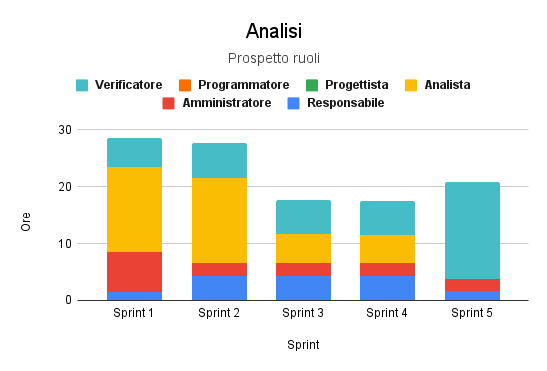
\includegraphics[scale=0.55]{../../assets/Diagrammi_Excel/Analisi.png}
	\end{minipage}
\hfill
	\begin{minipage}[c]{0.3\textwidth}
		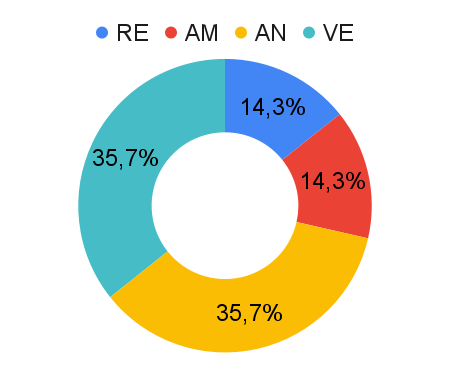
\includegraphics[scale=0.32]{../../assets/Diagrammi_Excel/Rip_An.png}
	\end{minipage}
	\caption{Prospetto ruoli per i vari sprint e ripartizione percentuale oraria}
\end{figure}



%------------------------------------------------------------------------------------
\newpage

\subsection{Technology Baseline}
Di seguito vengono riportate le tabelle orarie ed i costi relativi associati per la fase di Technology Baseline.

\begin{table}[h!]
	\footnotesize
\begin{minipage}[c]{0.53\textwidth}
	\centering
    \begin{tabular}{>{\raggedright\arraybackslash}c|cccccc|c}
    \rowcolor[RGB]{33, 73, 50}
    \multicolumn{1}{>{\centering\arraybackslash}c|}{\textcolor{white}{\textbf{Componente}}} 
        & \multicolumn{1}{>{\centering\arraybackslash}c}{\textcolor{white}{\textbf{RE}}} 
        & \multicolumn{1}{>{\centering\arraybackslash}c}{\textcolor{white}{\textbf{AM}}}
		& \multicolumn{1}{>{\centering\arraybackslash}c}{\textcolor{white}{\textbf{AN}}}
		& \multicolumn{1}{>{\centering\arraybackslash}c}{\textcolor{white}{\textbf{PT}}}
		& \multicolumn{1}{>{\centering\arraybackslash}c}{\textcolor{white}{\textbf{PG}}}
		& \multicolumn{1}{>{\centering\arraybackslash}c}{\textcolor{white}{\textbf{VE}}}
		& \multicolumn{1}{>{\centering\arraybackslash}c|}{\textcolor{white}{\textbf{Tot.}}}\\[4pt]
		
		\rowcolor[RGB]{216, 235, 171}
	    	Barilla Gianmarco & - & - & - & - & - & -& -		\\[4pt]
	    \rowcolor[RGB]{233, 245, 206}
	    	Beni Valentina & - & - & - & - & - & -& -			\\[4pt]
	    \rowcolor[RGB]{216, 235, 171}
	    	Bustaffa Marco & - & - & - & - & - & -& -			\\[4pt]
        \rowcolor[RGB]{233, 245, 206}
	    	Canel Alessandro & - & - & - & - & - & -& -			\\[4pt]
        \rowcolor[RGB]{216, 235, 171}
	    	Ferrarini Alessio & - & - & - & - & - & -& -		\\[4pt]
        \rowcolor[RGB]{233, 245, 206}
	    	Pozzebon Samuele & - & - & - & - & - & -& -			\\[4pt]
		\rowcolor[RGB]{47, 106, 73}
			\textcolor{white}{Totale Ruolo} & \textcolor{white}{10} & \textcolor{white}{8} & \textcolor{white}{7} 
			& \textcolor{white}{20} & \textcolor{white}{17} & \textcolor{white}{15}
			& \textcolor{white}{77} \\[4pt]	
    \end{tabular}
    \caption{Distribuzione delle ore nella fase di Technology baseline}
\end{minipage}
\hfill
\begin{minipage}{0.33\textwidth}
	\centering
	\begin{tabular}{cccc}
	    \rowcolor[RGB]{33, 73, 50}
	    \textcolor{white}{\textbf{Ruolo}} & \textcolor{white}{\textbf{Ore}} & \textcolor{white}{\textbf{Costo}}\\[4pt]
	    \rowcolor[RGB]{216, 235, 171}
	    Responsabile & 10 & 300\euro\\[4pt]
	    \rowcolor[RGB]{233, 245, 206}
	    Amministratore & 8 & 160\euro\\[4pt]
        \rowcolor[RGB]{216, 235, 171}
	    Analista & 7 & 175\euro\\[4pt]
	    \rowcolor[RGB]{233, 245, 206}
	    Progettista & 20 & 500\euro\\[4pt]
        \rowcolor[RGB]{216, 235, 171}
	    Programmatore & 17 & 255\euro\\[4pt]
	    \rowcolor[RGB]{233, 245, 206}
	    Verificatore & 15 & 225\euro\\[4pt]
		\rowcolor[RGB]{47, 106, 73}
			\textcolor{white}{Totale} & \textcolor{white}{77} & \textcolor{white}{1615\euro}\\[4pt]	
    \end{tabular}	
	\caption{Costi relativi al preventivo orario}

\end{minipage}
\end{table}

\begin{figure}[h!]
	\centering
	\begin{minipage}[c]{0.4\textwidth}
    	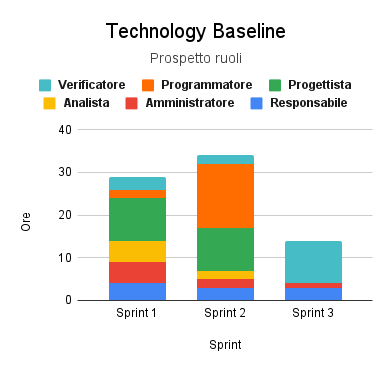
\includegraphics[scale=0.6]{../../assets/Diagrammi_Excel/Technology Baseline.png}
	\end{minipage}
\hfill
	\begin{minipage}[c]{0.4\textwidth}
		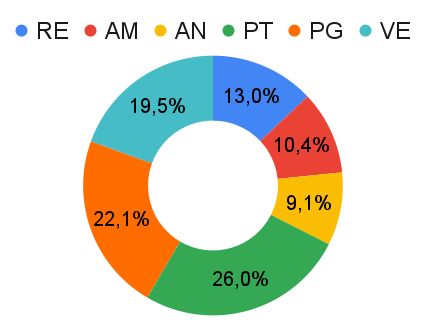
\includegraphics[scale=0.5]{../../assets/Diagrammi_Excel/Rip_tec.png}
	\end{minipage}
	\caption{Prospetto ruoli per i vari sprint e ripartizione percentuale oraria}
\end{figure}


\setlength\extrarowheight{0pt}